\documentclass[10pt,a4paper]{article}
%\usepackage{harvard}
\usepackage[margin=2cm, bottom=2cm]{geometry}
\usepackage{graphicx}
\usepackage{tabularx}
\usepackage{color}
\usepackage{caption}
\usepackage{subcaption}
\usepackage{tabu}
\usepackage{gensymb}
\usepackage{enumitem}
\usepackage{wrapfig}
\usepackage{algorithmic}

\captionsetup[figure]{labelfont=bf}
\captionsetup[table]{labelfont=bf}

\title{\vspace{-2em}Join Algorithms in SPARQL and their Scalability}
\author{pbqk24}
%\date{}

\begin{document}
	\maketitle
	
	\vspace{-3em}
	
	\section*{Abstract}
	% Summarise the project, including algorithms compared, measuring criteria, and the main results
	\section*{Introduction}
	The Semantic Web originated as a vision by Tim Berners-Lee that the web would be composed of structured and labelled data that could be directly parsed and processed by computers. Much progress has been made on turning this vision into a reality: for example, as of 2016 there were 2740 datasets implementing the principles of the Semantic Web, compared to only 1091 in 2014 \cite{Bizer}. Most of these datasets use RDF, the Resource Description Framework, to model the information and data stored in them. SPARQL is a query language for RDF, analogous to SQL for querying relational databases, which is used to retrieve data from RDF. Similarly to SQL, SPARQL implements several kinds of join algorithms in order to allow the combination of queries and data.
	
	As join algorithms are extensively used to build more complicated and useful queries, their implementation and efficiency is worthy of investigation. This will allow for analysis of the join algorithms, and the cost of using them in a query in terms of execution times. This project therefore investigates the scalability of two different join algorithms in SPARQL, and compares the join algorithms to their equivalents in SQL. The algorithms are being compared in terms of scalability with the number of joins performed, as well as the limit imposed on the number of results returned. This scalability is quantified in terms of wall-clock running time. %TODO SQL or not?
	
	% Set the scene, overview, motivation behind the work and choices
		% Brief overview of Semantic Web, RDF, SPARQL, their uses and why they are important
	% Overall description of what you did, main contributions
		% Analyse and compare the scalability of different join algorithms in SPARQL
	% How you are comparing algorithms, and how to measure the comparison
		% The algorithms are being compared in terms of their scalability, as well as their effect (i.e. what their effect is on the data/how they join data). This is measured in terms of wall-clock running time when ran on data on DBpedia. They are also compared to equivalent join operations in SQL
	
	\section*{Methodology}
	
	As stated above two join algorithms were investigated in this project. The first of these algorithms is conjunction, which is applied with the `.' operation in SPARQL. This takes two queries, and returns only those result that are present in the results of both queries, joining the results by matching the values of the common variables. This is equivalent to $A\cap B$, and is visualized in Figure \ref{inner_join}. The equivalent operation in SQL is inner join. This join algorithm was chosen because it is exceedingly common in SPARQL queries, as it is used to combine several queries to place multiple constraints on the return values. It therefore forms the building block of most complex queries.
		
	\begin{wrapfigure}{l}{0.3\textwidth}
		\vspace{-1em}
		\centering
		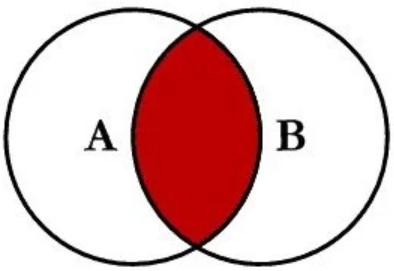
\includegraphics[width=0.3\textwidth]{figures/inner_join}
		\caption{Conjunction of two queries with `.'}
		\label{inner_join}
	\end{wrapfigure}

	A simple query was designed to use only this type of join in order to investigate the performance and scalability of this join algorithm. This query is shown in Figure \ref{alg:inner_join} in the appendix. This query searches for a person who has a name, has a gender, and has a partner who has a name and a gender also, and returns all of these objects. This query was shortened by removing queries and joins from the bottom, as well as editing the LIMIT set. For example, when investigating the use of only one join, the query simply searched for all people who have a name.
	
	The second join algorithm implemented in SPARQL is OPTIONAL, which takes two queries and returns all results from the first query, with results from the second query added (joined through matching the values of common variables) if they are found. The difference between conjunction discussed above and OPTIONAL is that the latter does not place a constraint on the existence of a match in the second query. IN SQL, the equivalent join algorithm is left join. This join algorithm was chosen as it is commonly used in SPARQL queries, for example being used in up to 50\% of queries submitted to DBPedia \cite{Atre}. It is extremely useful when querying semi-structured data found in RDF in order to retrieve data if it is found, but not place a requirement on it existing.
	
	The specific query used to investigate this join algorithm is shown in Figure \ref{alg:seq_left_join} in the appendix. This was constructed by replacing the conjunction operations in the first query with OPTIONAL operations. The full query selects all people, as well as their name, their gender, their partner, their partner's name, and their partner's gender, if they are found. As with the first query, this was modified by removing queries and OPTIONAL joins from the bottom, and by varying the LIMIT value. Additionally, for this join algorithm the impact of applying several joins nested instead of sequentially was also investigated. While these two approaches will result in different queries and as such are not interchangeable, it is potentially useful to investigate this difference. This query is shown in Figure \ref{alg:nested_left_join}.
	
	The queries used to investigate these join algorithms were constructed using \emph{yasgui.org}, an online GUI for writing and executing SPARQL queries on databases such as DBPedia. This was used to facilitate the development of the queries, as well as exploration of the data available on DBPedia. Performance metrics for the join algorithms were gathered using Python3 and the SPARQLWrapper library to repeatedly query DBPedia and collect wall-clock running times. This allowed for easier automation and repetition of experiments to produce more accurate and averaged data. Each query was performed 100 times, with each execution being individually timed. Then, the top 25\% of results were removed to account for outliers due to networking reasons, and the rest were averaged. The full code written for the data collection is attached in the appendix.
	
	These queries were designed to be simple to ensure a large amount of data would be available, to allow investigation of higher LIMIT values. Additionally, only the type of join being investigated was used in order to isolate the impact of each join algorithm in its respective experiment. Specifically, scaling with numbers of queries used was chosen as a metric as it can measure the impact using of the join algorithm in complex queries. This may for example inform a decision to simplify a query, or divide it into multiple, simpler queries to the dataset. Likewise scalability with the LIMIT value was chosen as this investigates the trade-off between performance and number of results to be returned. Knowledge of this trade-off could inform the decision between a more comprehensive but slower result, and a more efficient but potentially incomplete one. Thus, both these metrics have direct applications for the design of SPARQL queries.
	
	% Describe the algorithms and implementation details
		% Basic algorithm: Retrieve all persons that have a name
		% Augmented with additonal joins (inner joins) to filter data further: require a gender, require a spouse, require the spouse's name, require the spouse's gender
		% Second algorithm: same properties, but using OPTIONAL, i.e. retrieve all persons, list their name if they have one, list their gender if they have one, list their spouse if they have one, list their spouse's name if they have one, list their spouse's gender if they have one
		% These were implemented using an online SPARQL query GUI (yasgui.org) to facilitate development and exploration of the data. Performance metrics were gathered by using Python and the SPARQLWrapper library to repeatedly query dbpedia and collect wall-clock running times. This allowed for easier automation and repetition of experiments to get more accurate averaged data.
	% Include what measures you will measure the methods on
		% The methods are measured on wall-clock running times. As previously mentioned, this is done for several combinations of different scaling parameters (number of joins performed, limit imposed on the result). In the case of several outer joins, the case of sequentially applied joins vs nested joins is also investigated
	% Explain your choices
		% Inner join was chosen as the first algorithm because it is very commonly used in SPARQL queries in order to combine several groups of triples, e.g. to place several constraints on the return values (e.g. return each person, the person must have a name, the person must have a gender).
		% Optional is also extremely commonly used (used in up to 50% of queries submitted to DBPedia (https://www.cs.ox.ac.uk/people/medha.atre/papers/sigmod2015-atre.pdf)). It allows queries to return data if it is present, but not enforce the data's existence as a constraint, and thus is extremely useful in the semi-structured world of RDF.
	
	\section*{Results}
	
	The results for scalability of the inner join algorithm in SPARQL with number of joins performed and the LIMIT value is displayed in Figure \ref{fig:inner_join}. This graph shows a clear correlation between wall-clock running times and the number of join algorithms used, as well as with the LIMIT value used. This is expected, as the more join algorithms are used the more queries need to be executed and the results matched with the other queries. Likewise, as the LIMIT value is increased more results need to be found and matched against all the constraints placed in the form of the queries. These correlations hold for all values except for 3 joins and a LIMIT of 2000, which is higher than expected. This is likely an outlier caused by any of a range of factors: network connectivity, client-side network load, DBPedia load, etc.
	
	Notably, there is a much stronger increase in the running time as the number of join algorithms is increased than as the LIMIT value is increased. This is likely because for each additional join algorithm that is added, one additional query needs to be performed, and these results need to be matched against the rest. As the LIMIT value is increased, on the other hand, the same number of queries and matchings are performed, and only the process of selecting values to be returned is lengthened. The data does, however, suggest that the LIMIT value used affects the scaling with multiple join algorithms. For a LIMIT value of 2000 there seems to be a linear increase in running time as more joins are used, while for the highest LIMIT value tested, 4000, the increase seems to decay as more joins are introduced. However, this appearance of a pattern may also simply be caused by noise, which as previously discussed the data suffers from heavily.
	
	\begin{figure}[h!]
		\centering
		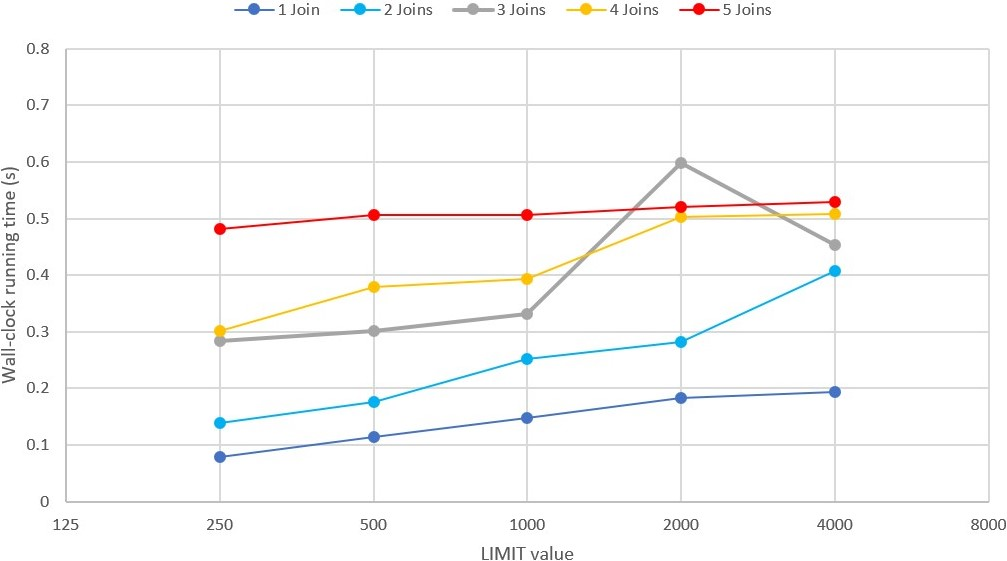
\includegraphics[width=0.8\textwidth]{figures/graph_inner_join}
		\caption{Wall-clock running times of inner join for varying numbers of joins performed and LIMIT values}
		\label{fig:inner_join}
	\end{figure}

	Figure \ref{fig:left_join} shows the results for the left join algorithm. Note that there is no data for five joins, as this query always resulted in a server timeout, and so no running time data could be gathered. Figure \ref{fig:seq_left_join}, which show the results for left joins applied sequentially, displays a clear correlation between the running time and the LIMIT value, and a weaker correlation to the number of joins applied. This is very different from what Figure \ref{fig:inner_join} shows for the inner join algorithm. This is likely because left join does not filter the results of the first query it is applied to, but rather adds data and results to it, while inner join filters out results from both queries. This means that simple OPTIONAL joins should be relatively easy to optimise behind the scenes, allowing the query engine to find as many results as requested first, and then execute the OPTIONAL queries only on this data, rather than the entire result of the first query, and still return correct results. This would explain the strong scaling with LIMIT value, as this increases the time taken for each query, and the weak scaling with numbers of joins performed. Again, this graph suffers from noise and some values which are likely to be outliers, such as the values for the query with three joins. As this entire query seems to have had lower running times than would be expected, this was likely caused by a temporary fall in server load or network activity.
	
	\begin{figure}[h!]
		\centering
		\begin{subfigure}[b]{0.45\textwidth}
			\hspace{-1cm}
			\centering
			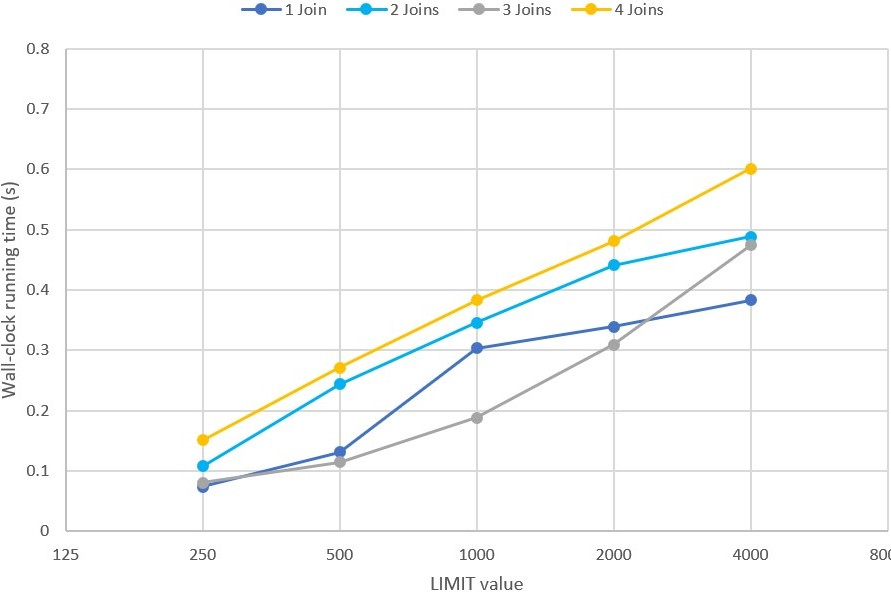
\includegraphics[width=1.1\textwidth]{figures/graph_sequential_left_join}
			\caption{Sequential Left Join}
			\label{fig:seq_left_join}
		\end{subfigure}
		\begin{subfigure}[b]{0.45\textwidth}
			\hspace{1cm}
			\centering
			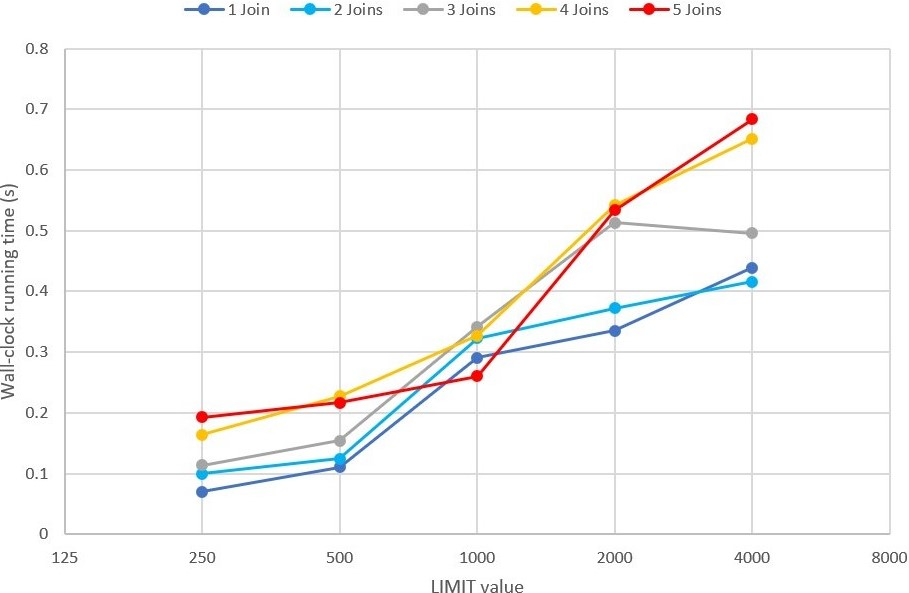
\includegraphics[width=1.1\textwidth]{figures/graph_nested_left_join}
			\caption{Nested Left Join}
			\label{fig:nested_left_join}
		\end{subfigure}
		\caption{Wall-clock running times of left join for varying numbers of joins performed and LIMIT values}
		\label{fig:left_join}
	\end{figure}

	Figure \ref{fig:nested_left_join} show the data gathered for nested left join algorithms. While this shows a correlation between running time and both LIMIT value and numbers of joins performed, the correlation is not as clear as for the other two experiments. In general, the data is very similar to that of the sequentially applied left joins, with the notable difference that the query with five left joins was successfully run when they were nested. Lastly, it is worth noting that the running times for the inner join queries were generally much higher for low LIMIT values than the queries with left joins, but lower or similar in value for higher LIMIT values.

	\section*{Conclusion}
	% What could you have done if you had more time
		% Investigate further/more complicated scalability cases, e.g. combination of inner and left joins.
		% Impact of query ordering on performance and scalability
		% Producing more accurate query wall-clock timings by querying a local database and tracking timings server-side, in order to remove impact of network speeds and congestion on results
	
	\begin{thebibliography}{9}
		\bibitem{Bizer}
		Bizer: Is the Semantic Web what we Expected? ISWC 2016, 10/20/2016 15th International Semantic Web Conference (ISWC 2016) Kobe, Japan, 10/20/2016 Is the Semantic Web what we Expected? Deployment Patterns and Data-driven Challenges Prof. Dr. Christian Bizer
		
		\bibitem{Atre}
		Medha Atre: OptBitMat: For SPARQL OPTIONAL left-outer-join queries, 2013 CoRR
	\end{thebibliography}

	\pagebreak
	\section*{Appendix}

	\subsection*{SPARQL Queries}

	\begin{figure}[h]
		\centering
		\begin{minipage}{0.5\textwidth}
			\begin{algorithmic}
				\STATE PREFIX dbo:\textless http://dbpedia.org/ontology/\textgreater
				\STATE PREFIX foaf: \textless http://xmlns.com/foaf/0.1/\textgreater
				\STATE SELECT *
				\STATE WHERE \{
				\STATE 	?person a dbo:Person .
				\STATE 	?person foaf:name ?name .
				\STATE 	?person foaf:gender ?sex .
				\STATE 	?person dbo:partner ?partner .
				\STATE 	?partner foaf:name ?partnername .
				\STATE 	?partner foaf:gender ?partnersex
				\STATE \}
				\STATE LIMIT 250
			\end{algorithmic}
			\caption{Inner Join Query}
			\label{alg:inner_join}
		\end{minipage}
	\end{figure}
	
	\begin{figure}[h]
		\begin{subfigure}[b]{0.5\textwidth}
			\begin{algorithmic}
				\STATE PREFIX dbo:\textless http://dbpedia.org/ontology/\textgreater
				\STATE PREFIX foaf: \textless http://xmlns.com/foaf/0.1/\textgreater
				\STATE SELECT *
				\STATE WHERE \{
					\STATE 	?person a dbo:Person
					\STATE 	OPTIONAL \{ ?person foaf:name ?name \}
					\STATE 	OPTIONAL \{ ?person foaf:gender ?sex \}
					\STATE 	OPTIONAL \{ ?person dbo:partner ?partner \}
					\STATE 	OPTIONAL \{ ?partner foaf:name ?partnername \}
					\STATE 	OPTIONAL \{ ?partner foaf:gender ?partnersex \}
					\STATE \}
				\STATE LIMIT 250
			\end{algorithmic}
			\caption{Sequential Left Join Query}
			\label{alg:seq_left_join}
		\end{subfigure}
		\begin{subfigure}[b]{0.5\textwidth}
			\begin{algorithmic}
				\STATE PREFIX dbo:\textless http://dbpedia.org/ontology/\textgreater
				\STATE PREFIX foaf: \textless http://xmlns.com/foaf/0.1/\textgreater
				\STATE SELECT *
				\STATE WHERE \{
					\STATE 	?person a dbo:Person
					\STATE 	OPTIONAL \{ ?person foaf:name ?name
					\STATE 	OPTIONAL \{ ?person foaf:gender ?sex
					\STATE 	OPTIONAL \{ ?person dbo:partner ?partner
					\STATE 	OPTIONAL \{ ?partner foaf:name ?partnername
					\STATE 	OPTIONAL \{ ?partner foaf:gender ?partnersex
					\STATE  \}\}\}\}\}
					\STATE \}
				\STATE LIMIT 250
			\end{algorithmic}
			\caption{Sequential Left Join Query}
			\label{alg:nested_left_join}
		\end{subfigure}
		
		\caption{Queries used to investigate the scalability of join algorithms in SPARQL}
		\label{queries}
	\end{figure}
	
	\subsection*{Python code}
	
\end{document}